\documentclass[12pt]{article} 
\usepackage[nohead]{geometry}
\usepackage[singlespacing]{setspace}
\usepackage[bottom]{footmisc}
\usepackage{indentfirst}
\usepackage{multirow}
\usepackage{amsmath, amssymb,amsfonts}
\usepackage{graphicx}
\usepackage[table]{xcolor}
\let\oldtabular\tabular 
\renewcommand{\tabular}{\large\oldtabular}
\usepackage{caption}
\usepackage{hyperref}
\hypersetup{
    pdftitle={FieldPaper},
    colorlinks=true,
    linkcolor=blue,
    filecolor=magenta,      
    urlcolor=cyan,
    citecolor=blue,
}
\urlstyle{same}
\usepackage{natbib}
\bibliographystyle{abbrvnat}
\setcitestyle{authoryear}
%\setlength\bibhang{0.5in}
\usepackage{float}

\newenvironment{proof}[1][Proof]{\noindent\textbf{#1.} }{\ \rule{0.5em}{0.5em}}
\newcommand{\pd}[2]{\frac{\partial#1}{\partial#2}}
\makeatletter
\def\@biblabel#1{\hspace*{-\labelsep}}
\makeatother
\geometry{left=1in,right=1in,top=1in,bottom=1in}


\title{Ethnic Enclaves and the Legacy of Internment}
\author{Dante Yasui}
\date{\today}

\begin{document}
\maketitle

\section{Intro}\label{intro}

\subsection{Research Question}\label{research-question}

\begin{itemize}

\item
  Did post-war relocation cause a permanent shift in the migration
  choices of Japanese Americans?
\end{itemize}

\begin{center}\rule{0.5\linewidth}{0.5pt}\end{center}

\subsection{Motivation}\label{motivation}

In the aftermath of Pearl Harbor over 100,000 Japanese Americans were subjected
to curfews, forced to assemble in temporary centers, and imprisoned in
internment camps from 1942 until the war's end. These families lost out on
years of earnings and education while also being forced to give up land and
belongings which they could not bring with them. The economic damages were
known to be large at the time, with the Japanese American Evacuation Claims Act
of 1948 leading to a total of \$148 million worth of claims on damage or lost
property and \$37 million actually being distributed
\citep{commission_on_wartime_relocation_personal_1983}. 
Because interned families also left behind their records, it is very difficult to know the
actual value of lost property. However, there is modern causal evidence that
West Coast Japanese suffered higher rates of mortality lower long-term earnings
\citep{chin_longrun_2005}, 
\citep{saavedra_early_2013},
and less educational attainment 
\citep{saavedra_school_2015} 
because of internment. 

Aside from the importance of understanding the losses to internees, Japanese
Internment can also serve as an interesting natural experiment through the
involuntary nature of the experiences of internees. One question asked by
previous economic literature is the extent that locations in which people live
affect their economic outcomes such as upward mobility or earnings. It is
difficult to provide an unbiased causal estimate because households usually
have a large degree of choice in where they live. Previous studies have used a
variety of empirical strategies to separate out this causal effect including
controlling for observable characteristics like education
\cite{glaeser_cities_2001}, worker fixed-effects \citep{card_location_2021}, or
through leveraging other exogenous placements of households like the Moving to
Opportunity Experiment (\cite{ludwig_long-term_2013},
\cite{chetty_effects_2016}, etc). 

\begin{itemize}
\item
  Immigrant populations tend to concentrate near places of initial
  settlement
\item
  Integration/assimilation could be important for immigrant labor market
  outcomes

  \begin{itemize}
  
  \item
    \cite{damm_ethnic_2009}
  \end{itemize}
\item
  Evidence for Canadian Japanese internment having persistant effect on
  spatial Japanese distribution
\item
  \cite{chan_forced_2022}
\end{itemize}

\subsection{Initial Distribution of pre-war Japanese
Population}\label{initial-distribution-of-pre-war-japanese-population}

\begin{center}
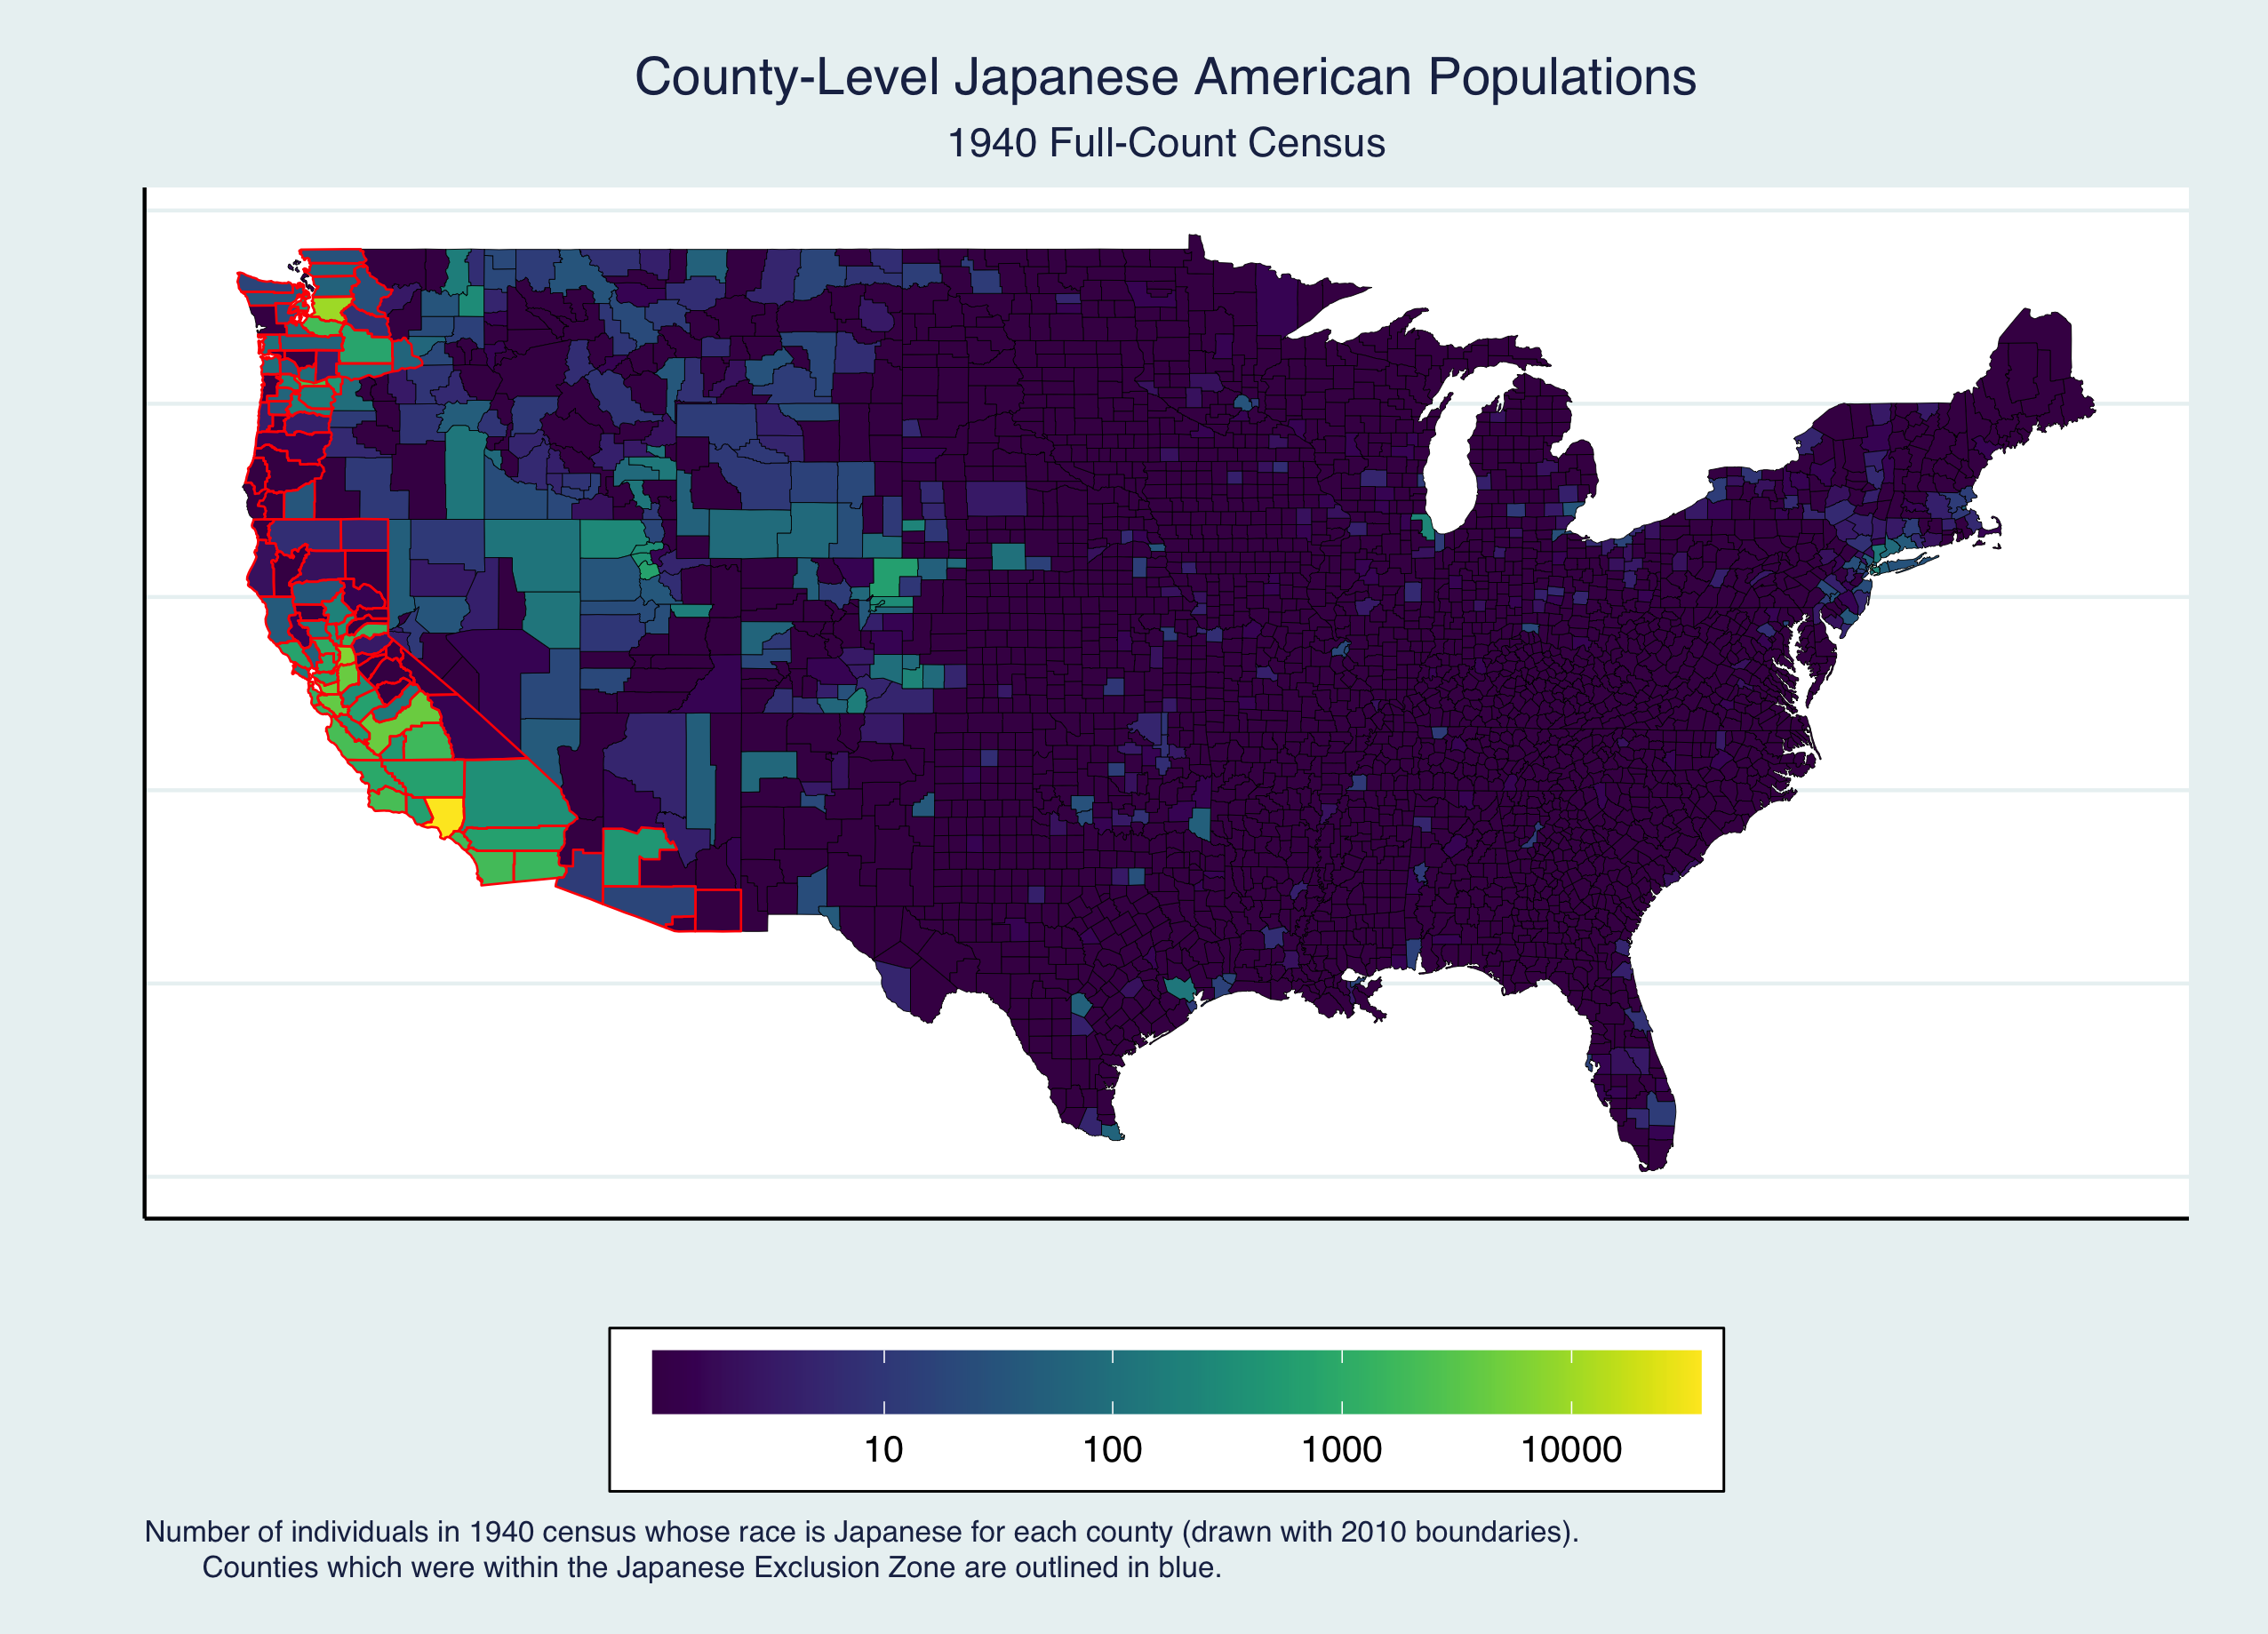
\includegraphics[width=1.0\textwidth]{figures/county_JAmap.png}
\end{center}


\section{Data}\label{data}

I combine historical census data, geographical references, and archived internment camp records to create the final pooled cross-section of county-year-level observations that I use in my later analysis. 

\subsection{Population and Migration}\label{population-and-migration}

For long-run migration data, I use the Decennial Census data provided by
the US Census Bureau via the
\href{https://usa.ipums.org/usa/index.shtml}{Integrated Public Use
Microdata Series} \citep{ruggles_ipums_2024}. The census
samples for which county locations are available include the 1940, 1950,
1980, and 1990 1\% samples, the 1960 5\% sample, and the 1970 Form 2
Metro 1\% sample.

One issue with comparing migration rates across years using census data is what and how migration questions were asked across different censuses.
1940 was the first year in which respondents were asked about their migration patterns with the specific questionnaire text
``In what place did this person live on April 1, 1935?''
However, in 1950 this question became
``Was [this household member] living in this same county a year ago?''
before switching back to asking about residence five years ago (instead of one) in all subsequent censuses.
\footnote{As documented in the IPUMS variable description page: \url{https://usa.ipums.org/usa-action/variables/MIGRATE5#description_section}}

Another problem with using 1950 responses to the migration question is that 
this census only this to `sample line' individuals, not to everyone.
Only one in every thirty people were asked about their location one year ago
in 1950 which drastically reduces the number of individuals who for which I can both 
identify their current county and previous county of residence within the public-use census data.

For the calculation of migration rates between counties, I define a
migrant as someone who reports that they either moved within the state,
between states, or that they were abroad five years ago (or in the past
1 year for 1960 respondents). This excludes people who report moving
within the same house, didn't report their previous location, or when their
location was reported as unknown.

\subsection{Geography}\label{geography}

\subsubsection{Historical County Borders}\label{historical-county-borders}

Although most county borders did not change much in the second half of
the 20th Century, there were counties which split, merged, or had name
changes which can make cross-decade comparisons difficult. For these
reasons, I use the county boundaries as they appeared in the 1990 census.

% *** Maybe include figure to show some counties changing over time?

To standardize historical county-level data to 1990 county definitions, I implement the crosswalk
method created by \cite{eckert_method_2020}. They overlay historical
county boundary shapefiles from \href{https://www.nhgis.org/}{NHGIS}
onto county boundaries for a specific target year (in this case 1990).
The sub-areas created by these overlays are used to calculate a set of
geographic weights which represent the fractions of a 1990 county's area
which were within the geographic areas of counties as they appear in
different decades (specifically the decades between and including 1940
to 1980). For my analysis, I take the crosswalk weights from the example
csv file for the end year 1990 which is published on the authors'
\href{https://github.com/liang-jack-a/EGLP_Crosswalk/tree/master}{github
repository}.

For the actual geographics boundaries of 1990 counties, I download the US county boundary shapefiles for the \href{https://www.census.gov/geographies/mapping-files/time-series/geo/tiger-line-file.html}{2008 TIGER/Line} basis from \url{nhgis.org} via the IPUMS NHGIS extract system.

I limit my data set to counties within the continental US, as Alaska and Hawaii were not yet states in 1940 and also because the effect of physical distance on migration is likely different for non-contiguous land areas.


\subsubsection{Camp Locations}\label{camp-locations}

Locations for historical interment camp locations were originally archived by
\href{http://encyclopedia.densho.org/War_Relocation_Authority/\#Planning_the_Camps}{Densho
Encyclopedia} and I downloaded these records in csv form via the
\href{https://www.arcgis.com/home/item.html?id=69183af8d45d4f46a9dc4eba99440891}{Behind
Barbed Wires} story project's website
(\cite{chrkan_behind_2019}, \cite{robinson_war_2023}).

I use the \texttt{sf} package in \texttt{R} to georeference the latitude-longitude coordinates from these records and project them to the same Coordinate Reference System used for the NHGIS shapefiles \citep{pebesma_simple_2018}.
\footnote{NHGIS uses the Contiguous Albers Equal Area Conic projection.}
This allows me to use the \texttt{st\_distance} function to obtain the distance matrix between all county-camp pairs and then select the closest camp to each county and the associated distance for my main independent variable.

\begin{figure}[H]
    \centering
    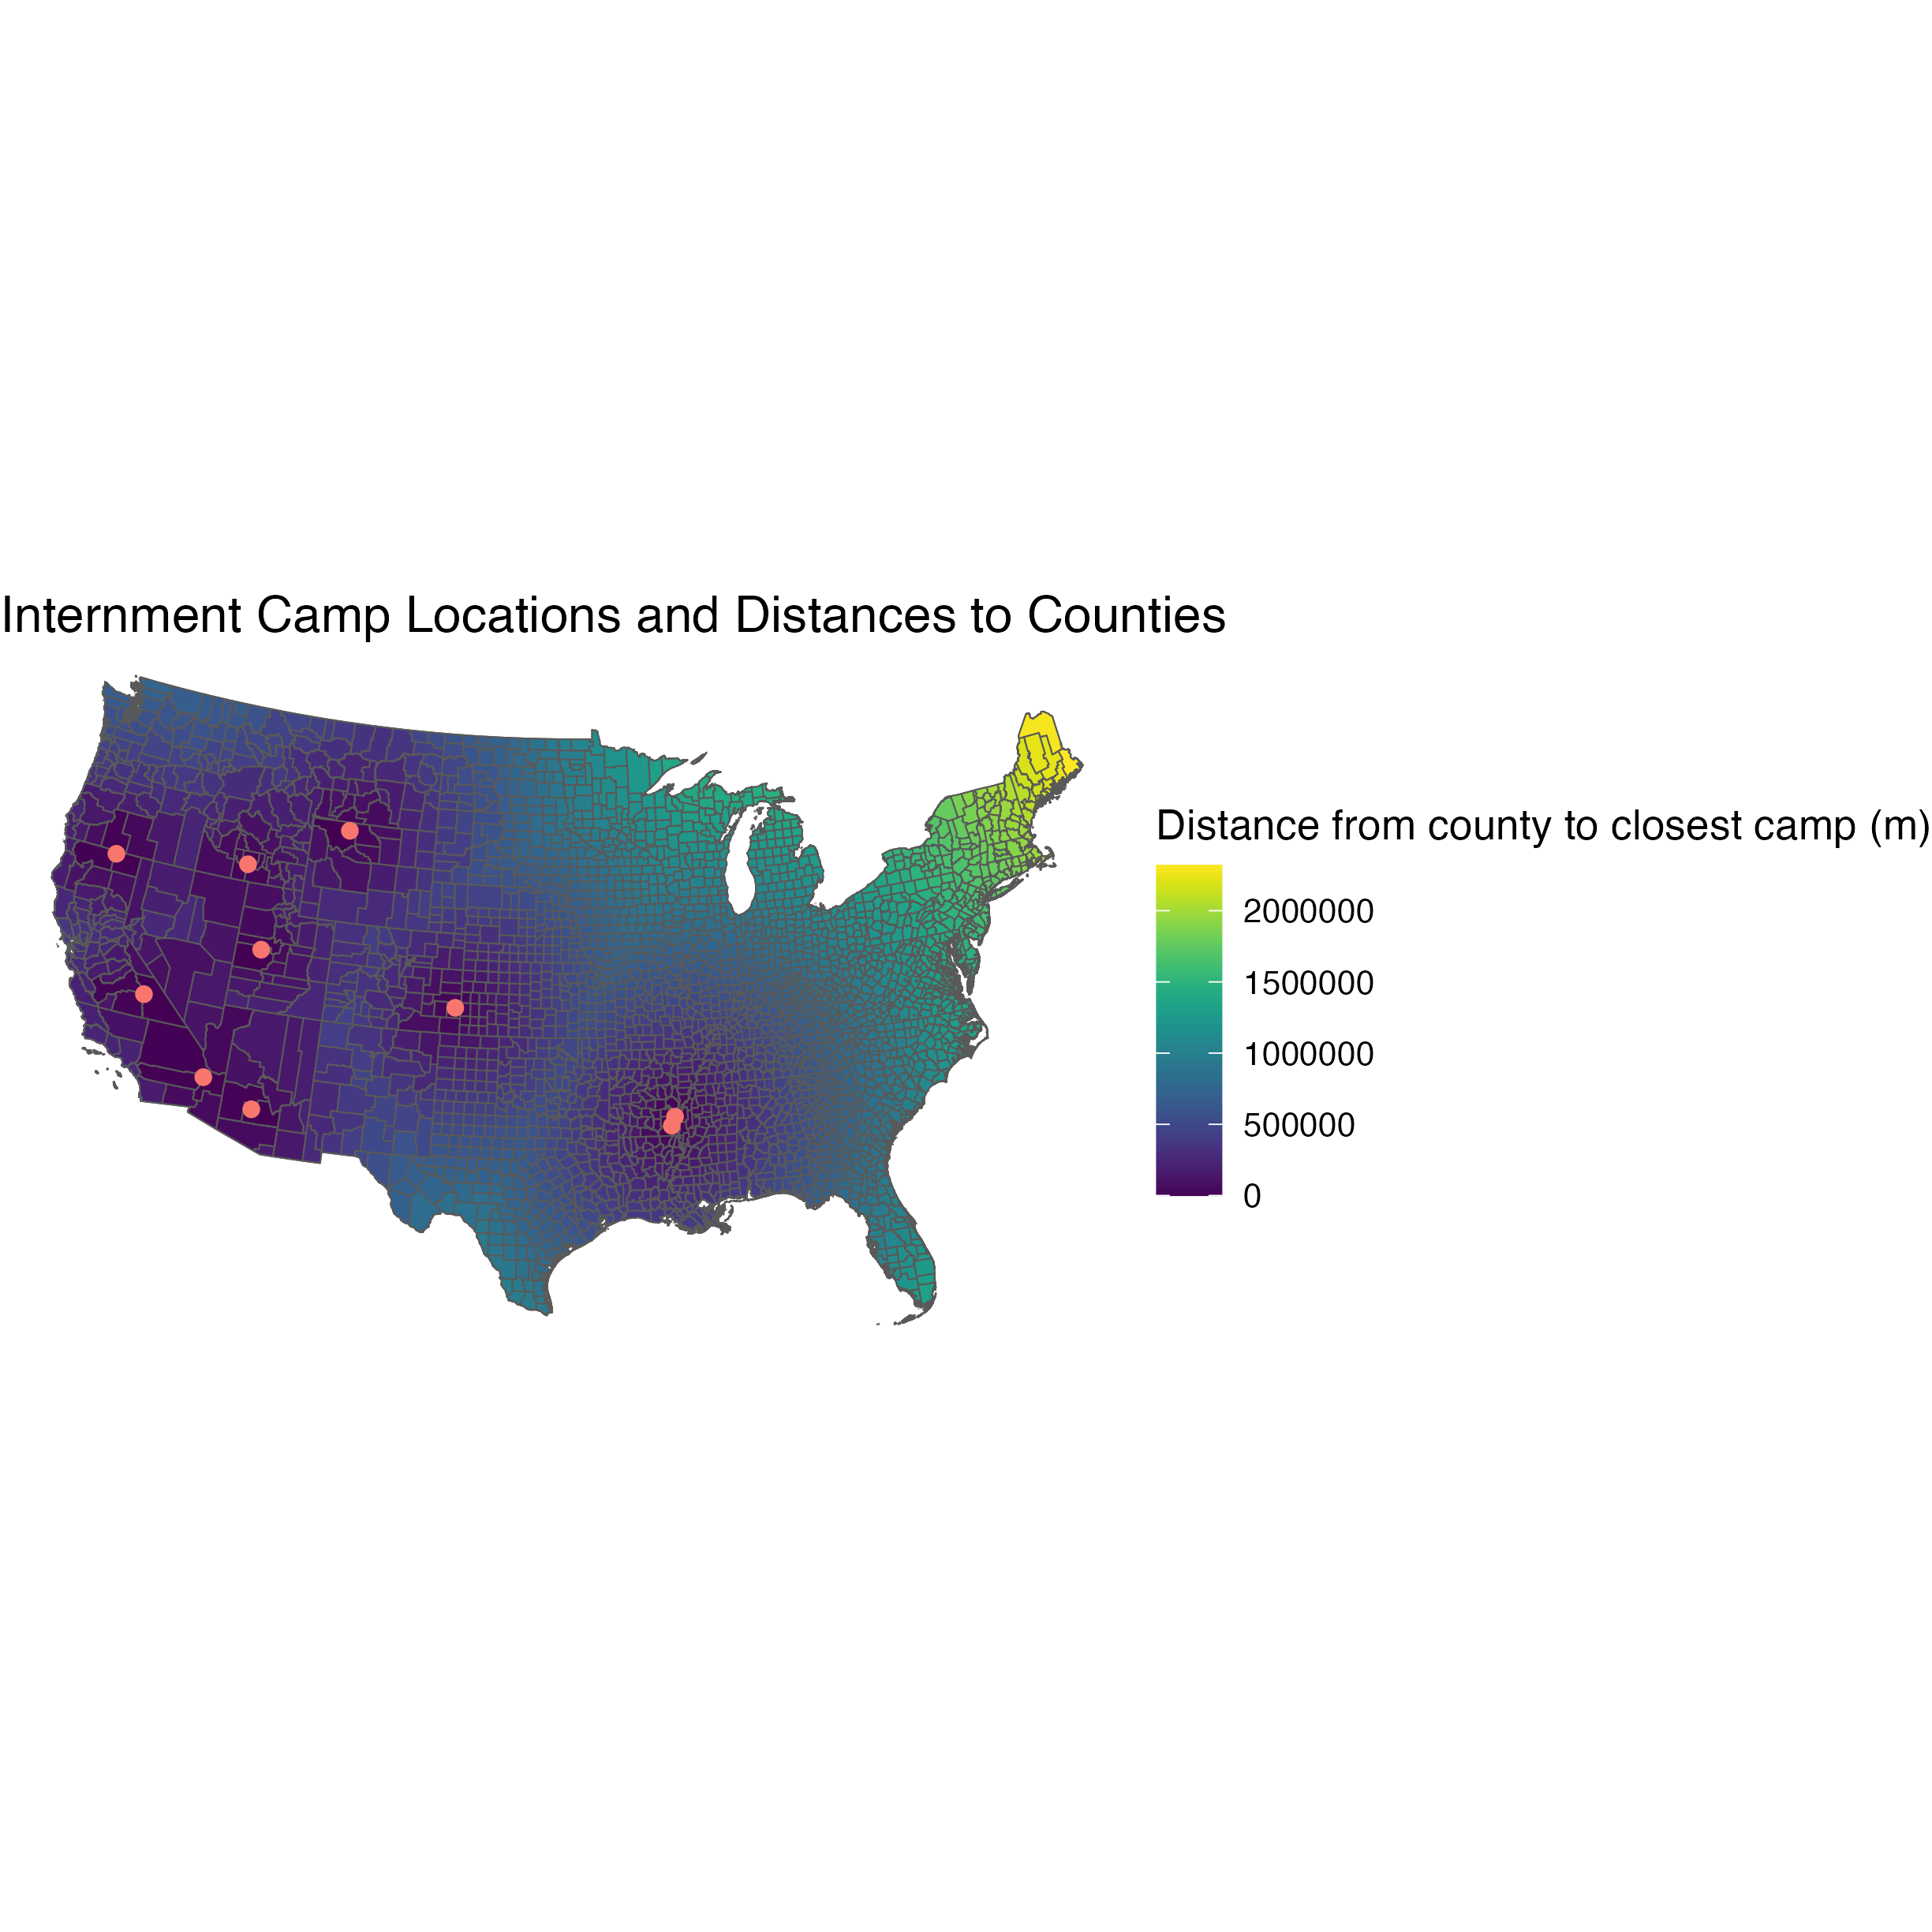
\includegraphics[width=1.0\textwidth]{figures/countymap.png}
    \caption{WRA internment camp locations with 1990 counties and their distances to each camp}
    \label{fig:countymap}
\end{figure}

Figure \ref{fig:countymap} shows the relationship between the internment camp locations and county boundaries. 
Each of the red dots represents the historical location of one of the ten WRA internment camps. 
From West to East they are:
Tule Lake and Manzanar, California;
Gila River, Arizona;
Minidoka, Idaho;
Topaz, Utah;
Heart Mountain, Wyoming,
Amache, Colorado;
and
Jerome and Rohwer, Arkansas.

\subsection{Historical counties
dataset}\label{historical-counties-dataset}

% Table created by stargazer v.5.2.3 by Marek Hlavac, Social Policy Institute. E-mail: marek.hlavac at gmail.com
% Date and time: Wed, Sep 18, 2024 - 16:34:32
\begin{table}[!h] \centering 
  \caption{County-Year Summary Statistics} 
  \label{ctysumstats} 
\begin{tabular}{@{\extracolsep{5pt}}lccccc} 
\\[-1.8ex]\hline 
\hline \\[-1.8ex] 
Statistic & \multicolumn{1}{c}{N} & \multicolumn{1}{c}{Mean} & \multicolumn{1}{c}{St. Dev.} & \multicolumn{1}{c}{Min} & \multicolumn{1}{c}{Max} \\ 
\hline \\[-1.8ex] 
Population & 4,257 & 132,663 & 356,496 & 0 & 7,495,400 \\ 
New Migrants & 4,257 & 53,316 & 148,182 & 0 & 3,216,300 \\ 
Migrant/Pop Ratio & 4,257 & 0.47 & 0.16 & 0.00 & 1.47 \\ 
New Japanese American Migrants & 877 & 720 & 3,199 & 0 & 60,480 \\ 
Current Japanese Population & 877 & 2,036 & 10,507 & 0 & 191,000 \\ 
Japanese/Total Migration Ratio & 877 & 0.0043 & 0.0173 & 0.00 & 0.34 \\ 
Average Age & 4,257 & 29.85 & 5.69 & 0.00 & 63.92 \\ 
Percent Female & 4,257 & 0.48 & 0.08 & 0.00 & 1.00 \\ 
Average Wage & 4,257 & 1,824.29 & 3,819.30 & 0.00 & 25,127.07 \\ 
Unemployment Rate & 4,257 & 0.07 & 0.05 & 0.00 & 1.00 \\ 
Distance to Closest Camp & 4,252 & 779,219 & 466,578 & 0 & 2,318,914\\ 
\hline \\[-1.8ex] 
\end{tabular} 
\end{table} 


All county-level observations in my final dataset are created by first taking the weighted average of each variable across all individuals who have an identifiable address within any county 
using the \texttt{PERWT} variable from IPUMS. 
Then I use the crosswalk weights from section \ref{historical-county-borders} to match data from historical counties on to the set of 1990 counties. 

After narrowing down to counties which can be observed in each census
year and then translating the historical counties to 1990 county
boundaries, I am left with 4,257 county-year level observations with observable migration rates.
However, there are many fewer observations with any data on migrations specifically by Japanese Americans.
There are 91 counties in 1940, 23 in 1950, 268 in 1960, 106 in 1970, 175 in 1980, and 207 in 1990 for which non-missing values exist for Japanese/Total Migration Ratio.
This variable is the main outcome in my later analysis and is defined as the number of new Japanese American migrants into the county divided by the total number of new migrants.

\begin{figure}[!h]
    \centering
    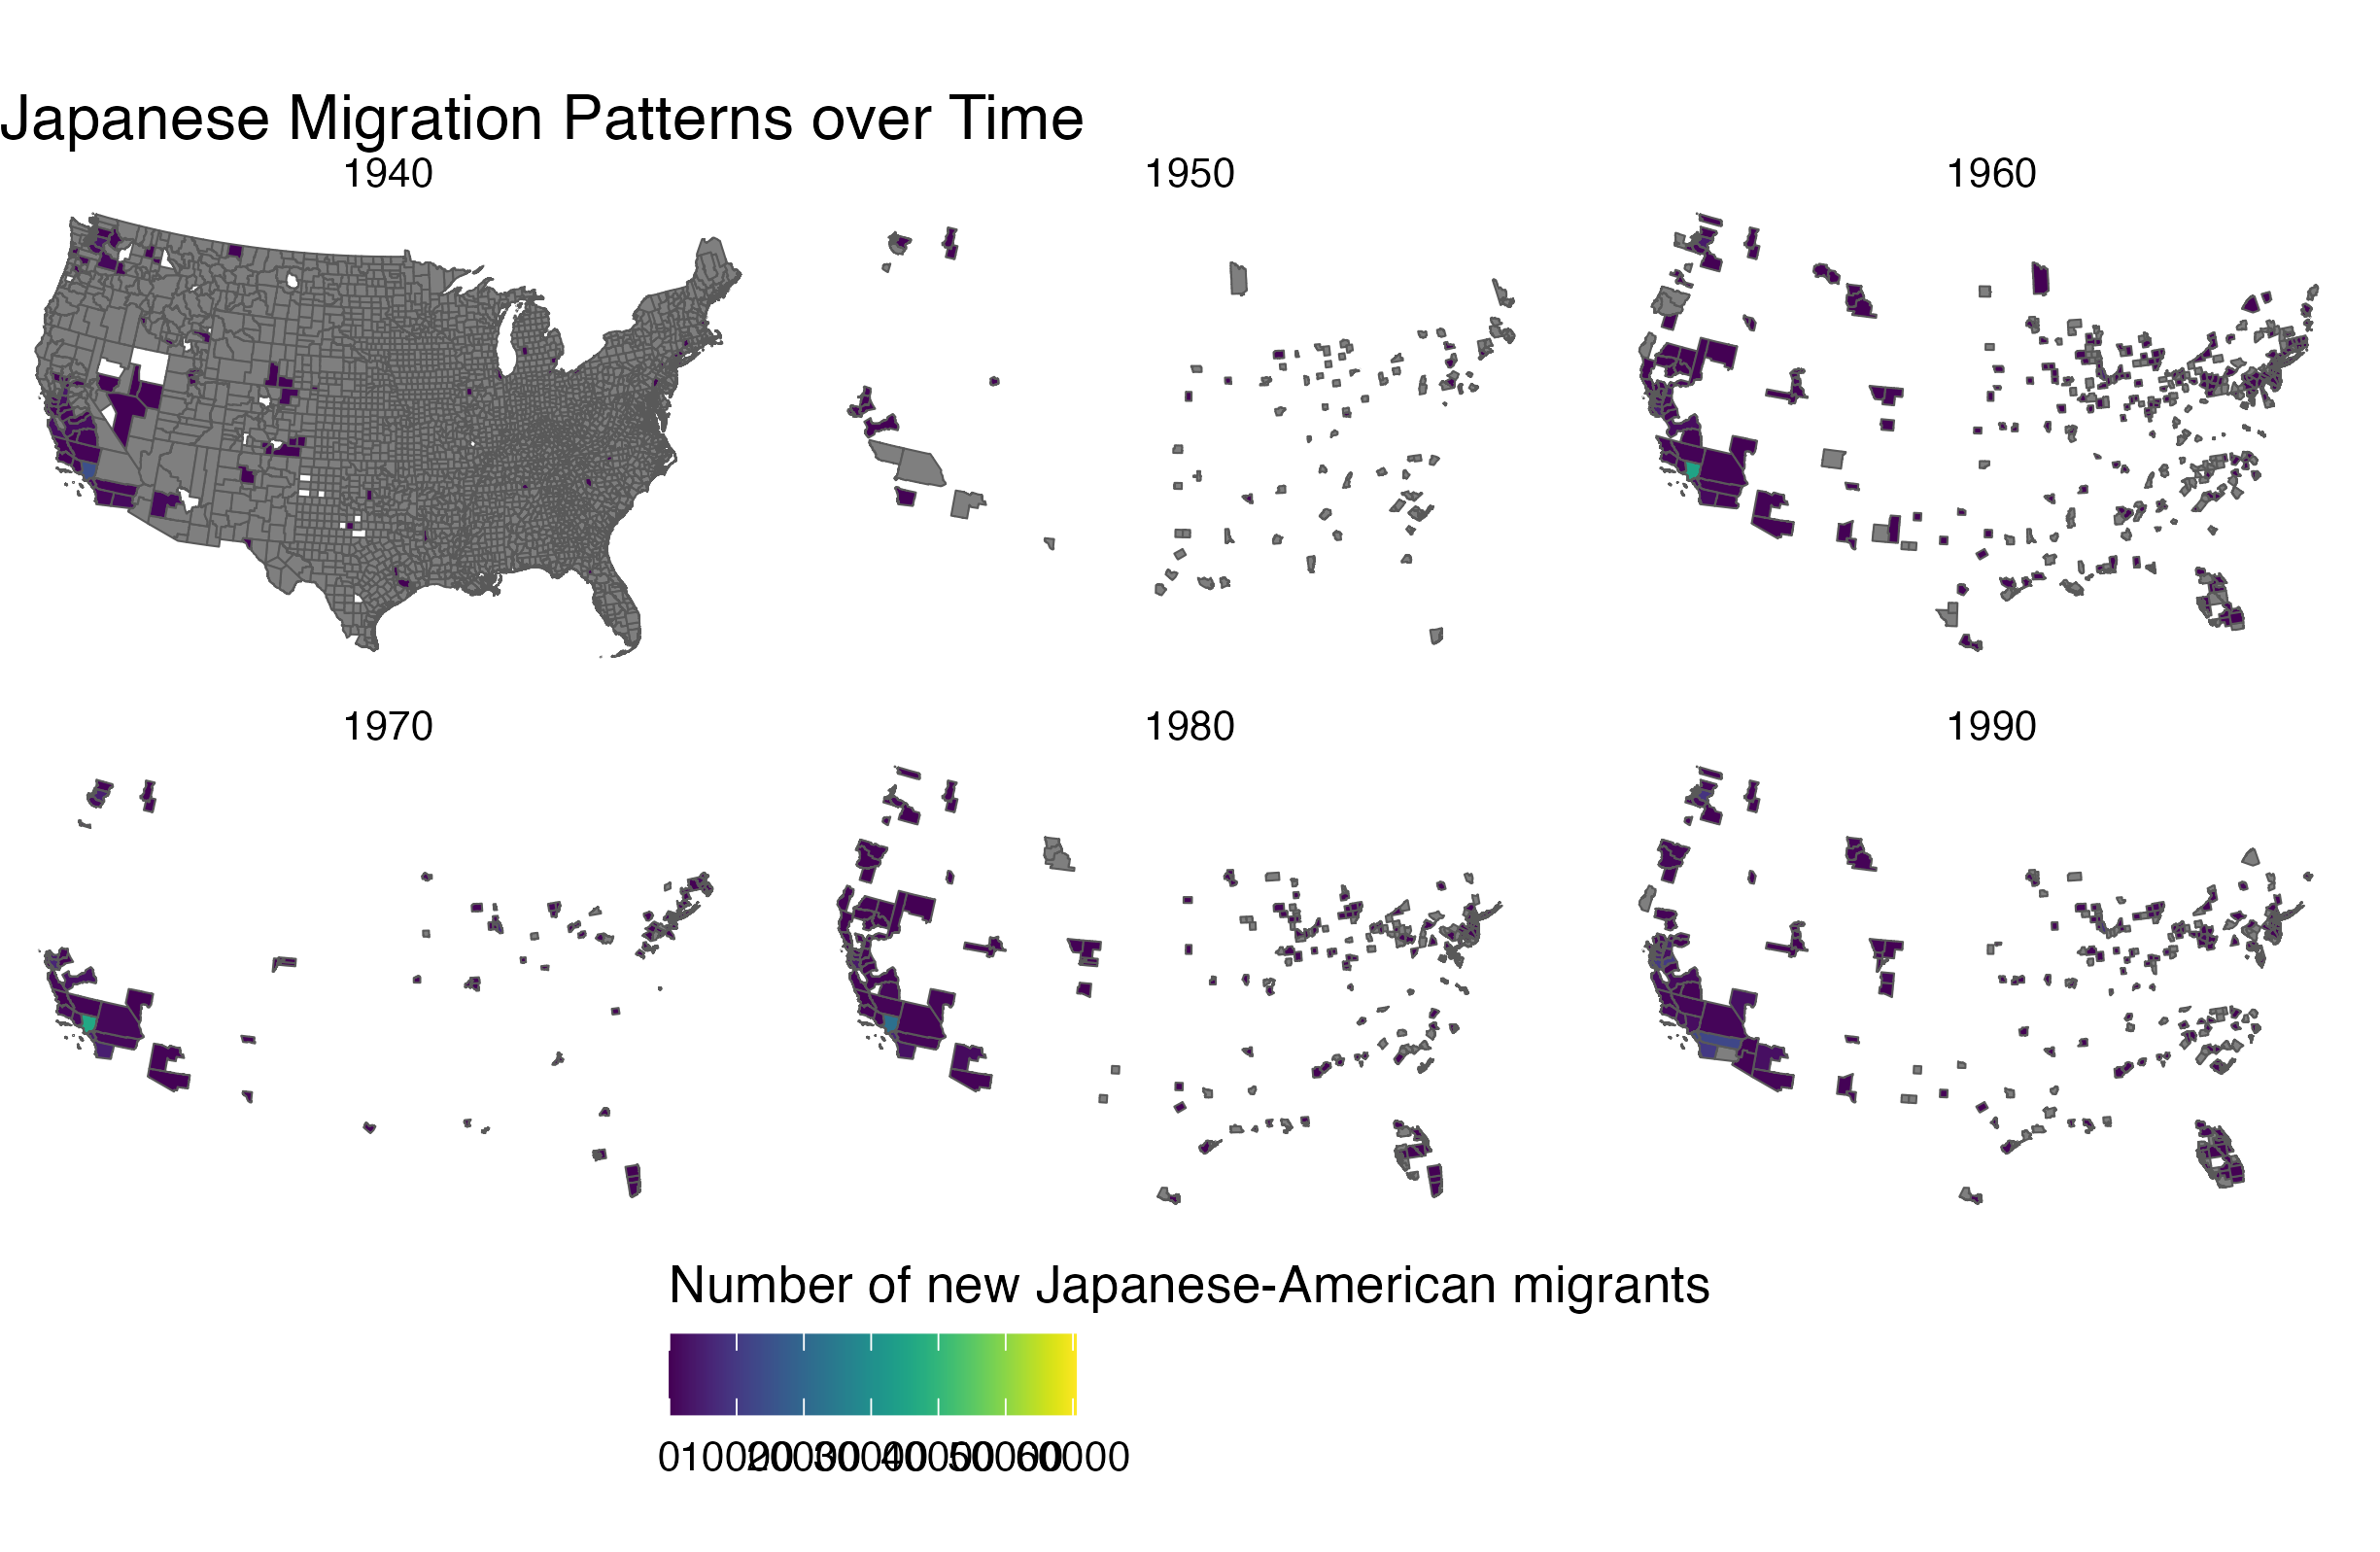
\includegraphics[width=1.0\linewidth]{figures/migrationmap.png}
    \caption{Japanese American migrations observable in each county for each census year}
    \label{fig:migrationmap}
\end{figure}

Figure \ref{fig:migrationmap} displays only the county-year observations for which there is any data available for any Japanese Americans who report moving into that county recently. 

\subsubsection{Representation of this Dataset}

The Census Bureau confidentiality standards state that public-use
microdata cannot report locations with populations of less
than 100,000 people. For this reason, many sparsely-populated counties
will be omitted from my sample because there are not enough observations
for the Census to report locations of individuals living there.


\phantomsection\label{cell-fig-comparesamplepops}
\begin{figure}[H]
\centering{
 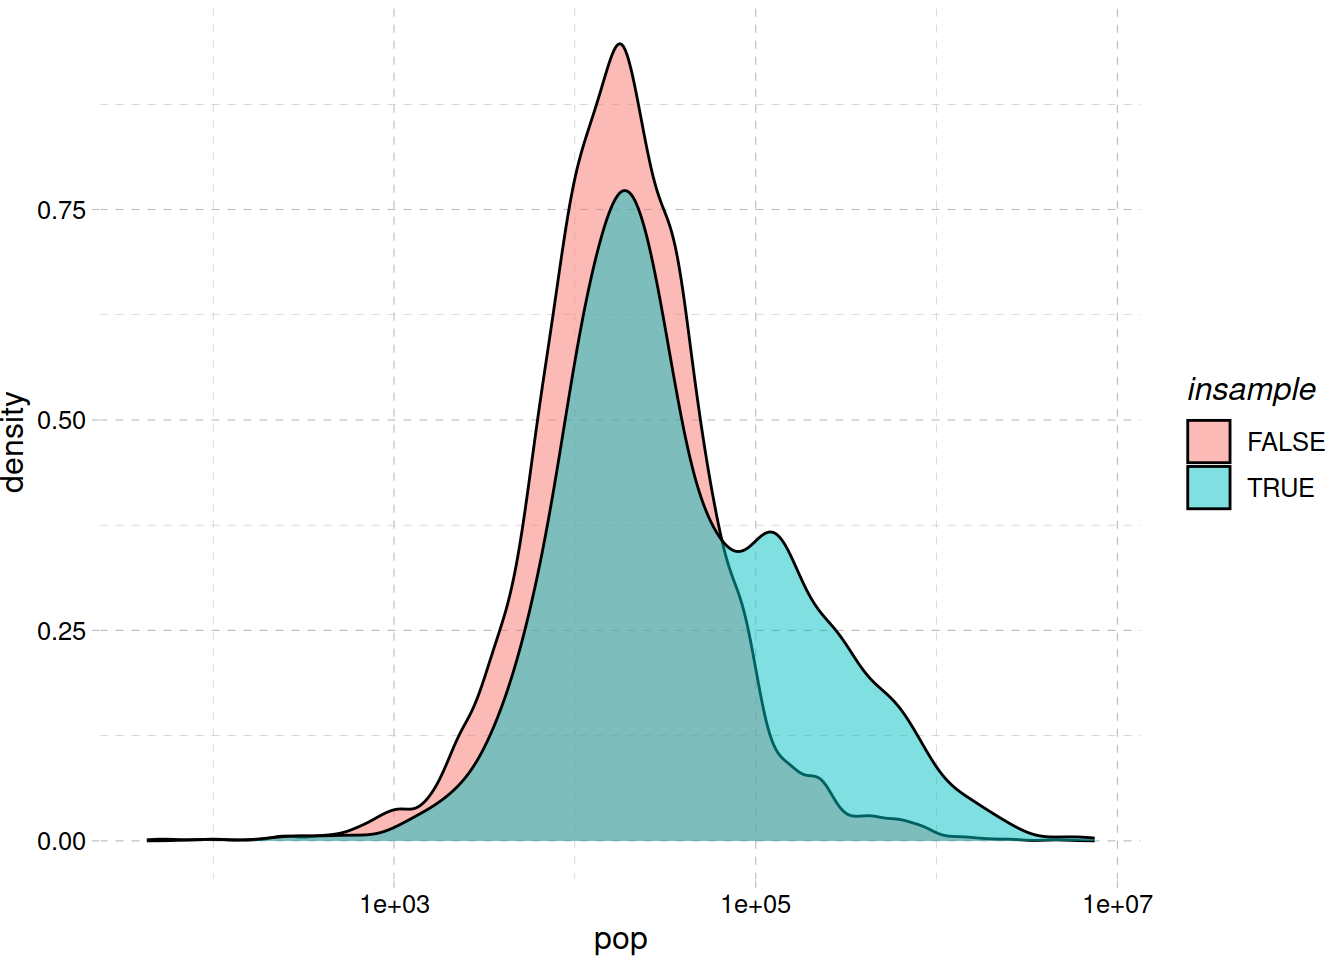
\includegraphics[width=.8\textwidth]{figures/fig-comparesamplepops-1.png}
}
\caption{\label{fig-comparesamplepops}County-year level population
distributions for identifiable (insample = TRUE) and for counties which are not in the final sample (insample = FALSE)}
\end{figure}%

The average population of the census-year observations in my sample is
133,000 while the average population for
crosswalked census-year observations outside my sample is
3,930,000. The fact that my sample is not
fully representative of all county sizes will be a challenge for the
external validity of my findings to extrapolate my results to smaller
counties for which I have less information on. However,
Figure~\ref{fig-comparesamplepops} shows that two different densities of
county-year populations observed in and out of the main sample have
similar shapes with the exception of a larger right-tail in the
in-sample density plot. This reflects the fact that counties with
populations of greater than 100,000 meet the Census Bureau's
confidentiality criteria, while data from smaller counties are subject
to stricter confidentiality measures.

\section{Methods}\label{methods}

To see whether the placement of camps during internment lead to any changes in the patterns of Japanese migration within the continental US, I estimate the correlation between the distance to the closest camp from a county with the ratio of new immigrants who's race is Japanese. 

\begin{equation}\label{eq:basicreg}
    \frac{mig\_japn_{it}}{mig\_total_{it}} = \beta_{0t} + \beta_{1t} Log(Distance)_i  +  \epsilon_{it}
\end{equation}


Equation \ref{eq:basicreg} outlines the more basic version of this relationship. 
The outcome variable, $\frac{mig\_japn_{it}}{mig\_total_{it}}$, is the number of new Japanese migrants into county $i$ in census year $t$ divided by the total number of new migrants into county $i$ of any race.
The single independent variable, $Log(Distance)_i$, is the log of the distance in meters from county $i$ to the camp closest to that county.

The linear parameter $\beta_0$ represents the ratio of Japanese migrants that this model predicts for a county that contains a camp (mathematically with a distance of 1 meter).
The parameter $\beta_1$ is the estimated amount that the ratio of Japanese to all migrants would increase for each 1\% increase in distance of a county away from the closest camp.
$\epsilon_{it}$ is the county-year level error term.

This model will not return the true causal effect of camp placement on migration outcomes if the choice of where to put the camps was itself affected by existing patterns of Japanese demographics.
One possible source of reverse-causality could come from the fact that, as illustrated in figure \ref{fig:countymap},
WRA camps were constructed close to the West Coast where the majority of the Japanese American population were already living. 
This means that West Coast counties would more likely to see higher rates of migration of this existing population than counties where no prior communities exist even in the absence of internment. 

While I do not claim to establish an unbiased causal estimate in this paper, 
I do add another variable to somewhat account for the endogenous placement of internment camps in equation \ref{eq:ezreg}.

\begin{equation}\label{eq:ezreg}
    \frac{mig\_japn_{it}}{mig\_total_{it}} = \beta_{0t} + \beta_{1t} Log(Distance)_i + \beta_2 EZ_i + \beta_3 Log(Distance)_i * EZ_i +  \epsilon_{it}
\end{equation}

The variable $EZ_i$ is an indicator variable which is equal to 1 for counties within the Evacuation Zone and 0 otherwise.
$\beta_2$ represents the difference in expected migration rates between counties in and out of the Evacuation Zone.

*** Caveats/assumptions ***

\section{Results}\label{results}


% Table created by stargazer v.5.2.3 by Marek Hlavac, Social Policy Institute. E-mail: marek.hlavac at gmail.com
% Date and time: Wed, Sep 11, 2024 - 17:28:07
\begin{table}[!htbp] \centering 
  \caption{Effects of Distance to Closest Camp on Japanese Migration by Decade} 
  \label{} 
\begin{tabular}{@{\extracolsep{5pt}}lcccccc} 
\\[-1.8ex]\hline 
\hline \\[-1.8ex] 
 & \multicolumn{6}{c}{\textit{Dependent variable:}} \\ 
\cline{2-7} 
\\[-1.8ex] & \multicolumn{6}{c}{Ratio of Japanese American migrants to total migrants} \\ 
 & 1940 & 1950 & 1960 & 1970 & 1980 & 1990 \\ 
\\[-1.8ex] & (1) & (2) & (3) & (4) & (5) & (6)\\ 
\hline \\[-1.8ex] 
 log(campclosest\_dist) & 0.096 & 0.032 & $-$0.024 & $-$0.085 & $-$0.059 & $-$0.120 \\ 
  & (0.076) & (0.074) & (0.084) & (0.077) & (0.079) & (0.081) \\ 
  Constant & $-$1.237 & $-$0.319 & 0.506 & 1.367 & 1.011 & 1.895 \\ 
  & (1.099) & (1.061) & (1.210) & (1.113) & (1.139) & (1.172) \\ 
 \hline \\[-1.8ex] 
Observations & 548 & 553 & 499 & 512 & 492 & 537 \\ 
R$^{2}$ & 0.003 & 0.0004 & 0.0002 & 0.002 & 0.001 & 0.004 \\ 
Adjusted R$^{2}$ & 0.001 & $-$0.001 & $-$0.002 & 0.0004 & $-$0.001 & 0.002 \\ 
\hline 
\hline \\[-1.8ex] 
\textit{Note:}  & \multicolumn{6}{r}{$^{*}$p$<$0.1; $^{**}$p$<$0.05; $^{***}$p$<$0.01} \\ 
\end{tabular} 
\end{table} 


Table \ref{tbl:distreg} reports the OLS estimates from equation \ref{eq:basicreg}.
Each column represents the parameters for each decade year $t \in \{1940, 1950, 1960, 1970, 1980, 1990\}$.
The dependent variable is the ratio of new migrants into a county who are Japanese to the total number of new migrants, $\frac{mig\_japn_{it}}{mig\_total_{it}}$.
The first row contains the slope estimates for $\beta_1$ in each regression
and the second row contain the intercept estimates for $\beta_0$.

Before any interment or relocation occurred, there is already a statistically significant negative relationship between proximity to the locations where camps would be built.
In column (1), I estimate that a county located 10\% farther away from an interment camp site was already associated with about a .04 percentage point reduction in the proportion of new migrants who are Japanese.
\footnote{***Percentage point not percent change because the outcome is a ratio?}
For the set of 91 counties in this regression, that would mean that a county which is 5.64 km farther away from the average county had an additional .4 percentage points in the Japanese migration ratio.

This correlation decreases in magnitude for later decades, although the point estimates become more precise in later years where more counties are included.
For the 1950 observations this correlation switches direction, although because of the small sub-sample included for this year, the null hypothesis that this particular estimate is non-zero cannot be rejected at the 95\% confidence level.


% Table created by stargazer v.5.2.3 by Marek Hlavac, Social Policy Institute. E-mail: marek.hlavac at gmail.com
% Date and time: Mon, Sep 16, 2024 - 16:07:49
\begin{table}[!htbp] \centering 
  \caption{Effects of Distance to Closest Camp on Japanese Migration by Decade} 
  \label{ezdistreg} 
\begin{tabular}{@{\extracolsep{2pt}}lcccccc} 
\\[-1.8ex]\hline 
\hline \\[-1.8ex] 
 & \multicolumn{6}{c}{\textit{Dependent variable:}} \\ 
\cline{2-7} 
\\[-1.8ex] & \multicolumn{6}{c}{Ratio of Japanese American migrants to total migrants} \\ 
 & 1940 & 1950 & 1960 & 1970 & 1980 & 1990 \\ 
\\[-1.8ex] & (1) & (2) & (3) & (4) & (5) & (6)\\ 
\hline \\[-1.8ex] 
 Log(Distance) & $-$1.247$^{***}$ & 0.003 & $-$0.088$^{***}$ & $-$0.157$^{***}$ & $-$0.046 & $-$0.071$^{*}$ \\ 
  & (0.417) & (0.393) & (0.026) & (0.053) & (0.065) & (0.038) \\ 
  Evac. Zone (EZ) & $-$20.488$^{**}$ & $-$3.536 & $-$2.128$^{***}$ & $-$4.701$^{***}$ & $-$1.470 & $-$2.568$^{***}$ \\ 
  & (9.046) & (11.846) & (0.694) & (1.011) & (1.306) & (0.928) \\ 
  Log(Distance) * EZ  & 1.512$^{**}$ & 0.248 & 0.178$^{***}$ & 0.378$^{***}$ & 0.136 & 0.217$^{***}$ \\ 
  & (0.659) & (0.858) & (0.050) & (0.072) & (0.093) & (0.067) \\ 
  Constant & 18.508$^{***}$ & 0.422 & 1.343$^{***}$ & 2.431$^{***}$ & 0.824 & 1.238$^{**}$ \\ 
  & (5.850) & (5.665) & (0.370) & (0.776) & (0.947) & (0.548) \\ 
 \hline \\[-1.8ex] 
Observations & 92 & 23 & 268 & 106 & 175 & 208 \\ 
R$^{2}$ & 0.106 & 0.019 & 0.295 & 0.545 & 0.224 & 0.268 \\ 
Adjusted R$^{2}$ & 0.076 & $-$0.136 & 0.287 & 0.532 & 0.211 & 0.257 \\ 
\hline 
\hline \\[-1.8ex] 
\textit{Note:}  


& \multicolumn{6}{r}{$^{*}$p$<$0.1; $^{**}$p$<$0.05; $^{***}$p$<$0.01} \\ 
\end{tabular} 
\end{table} 


Table \ref{tbl:ezdistreg} includes the indicator variable for a county being located in a state subject to evacuation, $EZ$, as outlined in equation \ref{eq:ezreg}.
For counties in 1940 outside of where the Evacuation Zone would be established (EZ=0), there is a correlation of about .7 of a percentage point reduction in the ratio of Japanese to total migrants for every 1\% increase in distance away from internment camps.
However, for counties within the evacuation zone that correlation is only .01 percentage points and positive but not statistically difference from zero.
Holding distance constant, the difference in this migration ratio between counties within and outside of the EZ was -8.2 percentage points but not significantly distinguishable from zero.

Just like in the previous regression, no statistically significant coefficients can be estimated for in the 1950 regression.

For the two decades 1960 and 1970 post-internment, the negative correlation between distance to camp locations and Japanese migration rates seems to decrease in magnitude but remain significantly negative for counties outside of the EZ.
However, unlike the 1940 regression, for these two decades the null hypothesis test that the coefficients on both $EZ$ alone and also on the interaction of $EZ$ and Log distance are zero can be rejected.
This may be due to the larger number of observations available in those regressions, although the significance goes away in the 1980 and 1990 regressions.

Ignoring significance levels, the overall descriptive pattern across all of these years seems to be that counties within the evacuation zone experienced lower rates of Japanese to total migration than non-EZ counties while their distance to nearby camp locations had no effect on these migration rates (with potentially positive effects in 1960 and 1970).
However, for counties which were never subject to evacuation orders, 
closer proximity to nearby camps seems to predict higher prevalence of Japanese Americans moving into those counties proportional to all migrants.

\section{Discussion}\label{discussion}

My results from the analysis of Japanese Americans' migrations from 1940 to 1990 
point to a few general patterns related to the geography of this population's internment during World War II.
I first document well-known general pattern from before the war 
that the vast majority of mainland Japanese Americans lived along the West Coast 
and that the WRA camps were placed closer to areas which already had higher rates of Japanese migrations relative to total migrations.
While the WRA's objective was to move the West Coast Japanese population away from population centers and military targets,
the selection of the ten locations chosen for the interment camps was likely limited by the higher transportation costs associated with relocating internees farther away from the West Coast.
The statistically significant and negative correlation which appears in the 1940 column of both table \ref{tbl:distreg} and table \ref{tbl:ezdistreg}
likely is due to this endogenous spatial proximity between the existing 1940 Japanese population and the internment camp locations.

As I discuss in section \ref{population-and-migration}, 
because only sample-line individuals were asked about their migrations in 1950
my 1950 sample of counties with measurable migration ratios is too small 
to detect any meaningful results.
Because this census was conducted only a few years after the end of internment,
it is unclear whether the opposite signs of the coefficients reported in the 1950 columns 
are due to noise or whether this reflects some actual short-term adjustment of 
Japanese American migration patterns caused by relocation and internment.
With the recently released full-count 1950 census data, it could be possible to gather more data to test the hypothesis that 1950 migrations by Japanese Americans were systematically different than other years,
although even that sample still suffers from the problems of sample-line individuals and asking about one year instead of five.


\bibliography{bibliography}

\end{document}
